%% Journal of Web Semantics / Elsevier manuscript draft
%% Compile with: pdflatex main && bibtex main && pdflatex main && pdflatex main

\documentclass[final,5p,times,twocolumn]{elsarticle}

\usepackage[T1]{fontenc}
\usepackage[utf8]{inputenc}
\usepackage{amsmath,amssymb}
\usepackage{booktabs}
\usepackage{array}
\usepackage{tabularx}
\usepackage{multirow}
\usepackage{graphicx}
\usepackage{xcolor}
\usepackage{url}
\usepackage[hidelinks]{hyperref}
\usepackage{enumitem}
\usepackage{siunitx}
\usepackage{tikz}
\usetikzlibrary{arrows.meta,positioning,shapes.geometric,fit}

\journal{Journal of Web Semantics}
\biboptions{numbers,sort&compress}

\newcommand{\mims}{\mathrm{MIMS}}
\newcommand{\kg}{knowledge graph}
\newcommand{\KG}{Knowledge graph}
\newcommand{\nhanes}{NHANES}
\newcommand{\cskg}{CSKG}
\newcommand{\todo}[1]{\textcolor{red}{[TODO: #1]}}
\newcolumntype{Y}{>{\raggedright\arraybackslash}X}

\begin{document}

\begin{frontmatter}

\title{When Definitions Change Conclusions: An Auditable Knowledge Graph for Accelerometer Use in Cancer Survivorship Research}

\author[aff1]{\todo{First Author}\corref{cor1}}
\ead{\todo{corresponding.author@email}}
\author[aff1]{\todo{Second Author}}
\author[aff2]{\todo{Additional Author}}
\cortext[cor1]{Corresponding author.}

\address[aff1]{\todo{Department, Institution, City, Country}}
\address[aff2]{\todo{Department, Institution, City, Country}}

\begin{abstract}
The same cancer survivor can appear eligible, ineligible, active, or inactive depending on the accelerometer rule used to process the same underlying data. This is a practical reproducibility problem: valid wear rules, minimum day rules, body placement, source metric, and activity thresholds can change conclusions, yet these definitions are often stored in prose, tables, or scripts rather than as auditable data. Cancer survivorship makes the problem especially important because physical activity evidence informs health behavior research, intervention design, and interpretation of long term outcomes, while public survey cancer variables are often self reported. We built a reproducible pipeline and knowledge graph for adults with self reported cancer history in NHANES 2011--2014 wrist accelerometry, with comparison sources from PhysioNet steps and NHANES 2003--2006 hip ActiGraph data. The pipeline generated processed tables, executable valid day protocols, provenance, expert reviewed cancer terminology mappings, RDF resources, SHACL validation, and competency questions. Among 1,035 adults with self reported cancer history, 878 had daily and minute accelerometry. Three valid day rules changed eligible counts from 722 to 862, a maximum discordance of 16.2 percentage points. The pilot graph contained 9,324 triples and passed validation with zero failed checks. The study shows that accelerometer definitions should be treated as reviewable semantic objects before cancer survivorship data are reused in clinical, epidemiological, or AI workflows.
\end{abstract}

\begin{keyword}
Knowledge graphs \sep Semantic harmonisation \sep Accelerometry \sep Provenance \sep SHACL \sep Cancer survivorship \sep Reproducibility
\end{keyword}

\end{frontmatter}

\section{Introduction}
\label{sec:introduction}

A cancer survivor may wear the same accelerometer, produce the same minute by minute signal, and still be treated differently by two studies. One study may count the participant as eligible because it requires four days with at least ten hours of valid wake wear. Another may exclude the same participant because it requires a stricter rule. A third may describe activity using steps, while a fourth uses wrist MIMS or hip ActiGraph counts per minute. The data did not change. The methodological definition changed.

This is not a minor reporting detail. Accelerometer studies depend on choices about device placement, wear time, nonwear treatment, epoch or minute summaries, source metric, valid day criteria, and activity thresholds. These choices can determine who enters the analytic cohort and what an activity variable means. A label such as ``physical activity'', ``movement volume'', or ``valid wear'' can hide very different measurement assumptions. A hip counts per minute threshold should not be transferred to wrist MIMS. A step count should not be inferred from a MIMS value. A valid day rule should not be treated as background preprocessing when it decides participant inclusion.

The problem is especially important in cancer survivorship research. Physical activity is a major concern for people living with and after cancer because it is linked to function, fatigue, quality of life, cardiometabolic risk, and survivorship care guidance \cite{rock2022acs,schmitz2019exercise}. Cancer survivors are also clinically heterogeneous. Cancer type, treatment exposure, stage, recurrence status, age, comorbidity, neuropathy, sarcopenia, and fatigue can all affect both activity behavior and interpretation. In this setting, an apparently technical change in an accelerometer rule can alter the meaning of a clinically relevant comparison.

Public population datasets add a second layer of risk. NHANES is valuable because it combines public health survey data with accelerometry, but its cancer history variables are questionnaire responses. They are not cancer registry records, pathology reports, treatment records, staging variables, recurrence variables, or current disease status measures. A reusable resource for cancer survivorship research must therefore prevent two kinds of overinterpretation: overinterpreting accelerometer metrics as interchangeable, and overinterpreting self reported cancer history as a clinically verified cancer diagnosis.

Existing literature provides strong foundations but not a complete solution. Accelerometry research has shown that wear rules, device placement, processing criteria, and thresholds affect physical activity estimates \cite{troiano2008physical,freedson1998calibration,migueles2017accelerometer}. MIMS was introduced as an open movement summary for raw accelerometer data, and NHANES 2011--2014 studies use wrist MIMS summaries such as daily MIMS and peak 30 minute MIMS \cite{john2019mims,zheng2023mims,saelee2021percentiles}. In parallel, Semantic Web research provides knowledge graph methods for integration, provenance, data quality, and validation \cite{hogan2021knowledge,ji2022survey,noy2019industry,zaveri2016quality}. SOSA and PROV provide established patterns for observations and derivations \cite{janowicz2019sosa,moreau2015prov}.

The gap is that accelerometer definitions are rarely represented as queryable and validated semantic objects. They are usually written for human readers or embedded in analysis scripts. This makes it hard for reviewers, analysts, and AI systems to ask basic questions: which rule produced this feature, which participants change eligibility under another rule, which source metric is being used, which cancer terminology mapping was reviewed, and which harmonisation claims are explicitly blocked. Knowledge graph construction has also been studied extensively \cite{paulheim2017refinement,ristoski2016semantic}, but less attention has been given to representing negative domain knowledge such as ``do not convert'', ``do not infer'', and ``not a clinical diagnosis'' as first class evidence.

The aim of this paper is to build and evaluate an auditable semantic layer for accelerometer definitions in cancer survivorship research. We use adults with self reported cancer history in NHANES 2011--2014 wrist accelerometry as the primary case. We add a same cohort PhysioNet step source and an independent NHANES 2003--2006 hip ActiGraph source to test where harmonisation should stop. The purpose is not to create a new clinical activity classifier. The purpose is to make methodological definitions, provenance, terminology mappings, and interpretation limits explicit enough to be checked.

The study tests three expectations. First, different valid day rules will change the eligible cancer history cohort. Second, a knowledge graph can record the source and protocol behind each accelerometer feature. Third, the graph can make unsupported claims visible and blocked, including conversion from wrist MIMS to hip counts per minute, inference of steps from MIMS, and clinical diagnosis assertions from self reported cancer codes.

The contributions are:
\begin{enumerate}[leftmargin=*]
    \item a reproducible NHANES pipeline that connects self reported cancer history, wrist accelerometry, valid day protocols, derived features, and provenance;
    \item a semantic model that represents accelerometer definitions as auditable objects rather than hidden preprocessing decisions;
    \item a harmonisation model that records both allowed abstractions and blocked conversions across MIMS, steps, and hip counts;
    \item expert reviewed NCI Thesaurus mappings that remain qualified source code mappings rather than clinical diagnosis assertions;
    \item validation evidence from SHACL, policy guards, and competency questions showing that the graph can support reviewer audit.
\end{enumerate}

\section{Background and Related Work}
\label{sec:background}

\subsection{Why accelerometer definitions affect conclusions}

Accelerometers do not directly output a clinical activity state. They produce signals that become analytic variables only after processing decisions. Earlier large population studies used hip worn ActiGraph counts per minute and calibrated intensity thresholds \cite{troiano2008physical,freedson1998calibration}. Later reviews emphasized that collection and processing criteria, including wear time, nonwear definitions, epoch length, and cut points, can change physical activity and sedentary behavior estimates \cite{migueles2017accelerometer}. MIMS addresses part of this problem by providing an open monitor independent movement summary for raw accelerometer processing \cite{john2019mims}. However, a monitor independent movement summary is still not equivalent to steps, hip counts per minute, or an intensity classification.

The relevant methodological issue is therefore not only whether an accelerometer variable exists, but how that variable was produced and what conclusions it supports. A valid day rule can be compared as a completeness definition. A source metric can be stored as a measurement. An activity threshold can be applied only in the context for which it was defined or validated. These distinctions are easy to blur when harmonisation is performed by variable labels alone.

\subsection{Why cancer survivorship raises the stakes}

Cancer survivorship research often uses physical activity to study health behavior, rehabilitation, fatigue, function, and long term outcomes \cite{rock2022acs,schmitz2019exercise}. Misclassification can therefore affect more than a descriptive table. It can change which survivors appear to meet activity guidance, which subgroups appear at risk, and how interventions or observational associations are interpreted.

Cancer survivorship also requires careful terminology. A survey response indicating prior cancer is useful for public health research, but it is not the same as a registry confirmed cancer diagnosis. Broad cancer type labels may not define histology, stage, treatment, recurrence, or current disease status. For this reason, semantic harmonisation in this domain must preserve uncertainty and source limitations instead of turning every code match into a strong biomedical assertion.

\subsection{Knowledge graphs as audit infrastructure}

Knowledge graphs integrate data with explicit semantics and machine readable relations \cite{hogan2021knowledge,ji2022survey}. They are useful in complex settings because they can connect entities, source records, definitions, provenance, and validation evidence across heterogeneous data \cite{noy2019industry}. However, useful graph construction requires more than table conversion. It requires modelling choices, quality assessment, refinement, and governance \cite{paulheim2017refinement,zaveri2016quality}.

Sensor and provenance ontologies are particularly relevant. SOSA provides a lightweight pattern for sensors and observations \cite{janowicz2019sosa}, while PROV describes how entities are generated by activities and linked to sources \cite{moreau2015prov}. These patterns allow an accelerometer feature to be represented not as a free floating number, but as an observation or derived entity with a source, processing activity, protocol, and interpretation limit.

\subsection{Validation and semantic safeguards}

Operational knowledge graphs need validation. SHACL supports constraint checking over RDF graphs and has been studied formally in relation to satisfiability, containment, and recursion \cite{pareti2022recursive}. In this study, validation is used as a review gate. It checks that required graph properties exist and that domain rules are respected. The most important safeguards are negative: an unreviewed NCIt mapping must not enter as an asserted code mapping, a wrist MIMS variable must not inherit hip count thresholds, and a self reported cancer type must not become a registry confirmed diagnosis.

\section{Materials and Methods}
\label{sec:methods}

\subsection{Research question and study design}

The primary research question was: can a knowledge graph make accelerometer definitions auditable enough to explain and constrain different activity conclusions in cancer survivorship research? Three operational questions followed from this aim. First, how much do valid day rules change eligible participant counts among adults with self reported cancer history? Second, can processed accelerometer features be linked to their source files, protocols, and derived feature definitions? Third, can semantic safeguards block unsupported conversions and clinical overclaims?

The study used a quantitative and semantic engineering design. The quantitative component processed public accelerometer data and calculated cohort counts, valid day counts, eligibility, daily MIMS summaries, and source specific activity definition outputs. The semantic component represented the processed evidence as RDF, added provenance and review decisions, and validated the graph with SHACL, policy guards, and competency questions. This mixed design was selected because the research problem concerns both numerical results and the meaning of the definitions that produced those results.

\subsection{Data sources and cohort selection}

The primary source was NHANES 2011--2012 and 2013--2014. These cycles were selected because they include public wrist worn physical activity monitor data processed into MIMS units and questionnaire variables for cancer history. The cohort included participants aged 20 years or older with self reported cancer history, defined as MCQ220 = 1. SEQN was used as the participant key across demographic, medical condition, monitor header, day, and minute files.

Two additional public accelerometry sources were included to test harmonisation boundaries. PhysioNet ActiLife step summaries for NHANES 2011--2014 were used as a same cohort derived step source. NHANES 2003--2006 hip worn ActiGraph PAM minute data were processed as an independent public source that differs by cycle, participant set, placement, and metric. This second source supports a cross source test of metric compatibility, but it is not an independent clinical cancer survivorship registry.

Table~\ref{tab:cohort} reports cohort construction for the primary NHANES 2011--2014 wrist source.

\begin{table}[t]
\caption{Cohort construction for the primary NHANES 2011--2014 wrist accelerometry source.}
\label{tab:cohort}
\centering
\scriptsize
\begin{tabularx}{\columnwidth}{Yrrr}
\toprule
Stage & 2011--2012 & 2013--2014 & Total \\
\midrule
All participants & 9,756 & 10,175 & 19,931 \\
Age $\geq$ 20 years & 5,560 & 5,769 & 11,329 \\
Self reported cancer history & 488 & 547 & 1,035 \\
PAM header available & 462 & 530 & 992 \\
Daily PAM summary available & 406 & 472 & 878 \\
Minute level PAM data available & 406 & 472 & 878 \\
\bottomrule
\end{tabularx}
\end{table}

\subsection{Data preparation}

Source files were converted into processed tables before RDF generation. The processed layer included participants, cancer diagnosis slots, daily movement summaries, retained minute rows, derived minute features, protocol definitions, protocol application results, source manifests, source code mappings, NCIt review records, and validation reports. Participant records were checked for unique SEQN values. Diagnosis, day, and minute records were checked against participant identifiers so that orphan rows could not enter the graph.

The NHANES 2011--2014 minute files were processed in chunks because the retained records were large. The primary retained minute table contained 9,949,908 rows for the 878 participants with daily and minute accelerometry. Derived participant day features were calculated from minute rows and linked back to daily summaries. A tiny zero like value in the source files, 5.397605e-79, was treated as a zero like numeric artifact rather than a separate quality or biological state.

\subsection{Protocol definitions and calculations}

Three valid day rules were encoded as executable protocols (Table~\ref{tab:protocols}). The rules were selected to demonstrate how cohort membership changes when the minimum daily wear requirement changes. Each rule required at least four valid days per participant. The protocols are completeness rules only. They do not classify a participant as active, inactive, sedentary, or meeting MVPA recommendations.

\begin{table}[t]
\caption{Executable valid day protocols represented in the graph.}
\label{tab:protocols}
\centering
\scriptsize
\begin{tabularx}{\columnwidth}{>{\raggedright\arraybackslash}p{0.34\columnwidth}Y>{\raggedright\arraybackslash}p{0.23\columnwidth}c}
\toprule
Protocol & Definition & Condition & Days \\
\midrule
\shortstack[l]{\texttt{wake\_wear}\\\texttt{10h\_min4}} & At least 10 h valid wake wear & \texttt{PAXWWMD >= 600} & 4 \\
\shortstack[l]{\texttt{wake\_wear}\\\texttt{12h\_min4}} & At least 12 h valid wake wear & \texttt{PAXWWMD >= 720} & 4 \\
\shortstack[l]{\texttt{valid\_minutes}\\\texttt{20h\_min4}} & At least 20 h valid data & \texttt{PAXVMD >= 1200} & 4 \\
\bottomrule
\end{tabularx}
\end{table}

For each participant and protocol, a day was marked valid when the condition was true. A participant was marked eligible when the valid day count was at least four. The pipeline calculated observed days, valid days, eligibility status, total MIMS, mean participant daily MIMS, peak 30 minute MIMS, eligible participant counts, eligible percentages, and pairwise inclusion discordance between protocols.

\subsection{Knowledge graph construction}

The graph was generated after tabular quality checks passed. Each participant, self reported cancer history assertion, cancer diagnosis slot, sensor, daily movement summary, minute observation, feature set, processing protocol, protocol result, citation evidence node, activity data source, harmonisation mapping, and independent source summary was represented as an RDF resource. Figure~\ref{fig:pipeline} summarizes the workflow.

\begin{figure*}[t]
\centering
\resizebox{0.92\textwidth}{!}{%
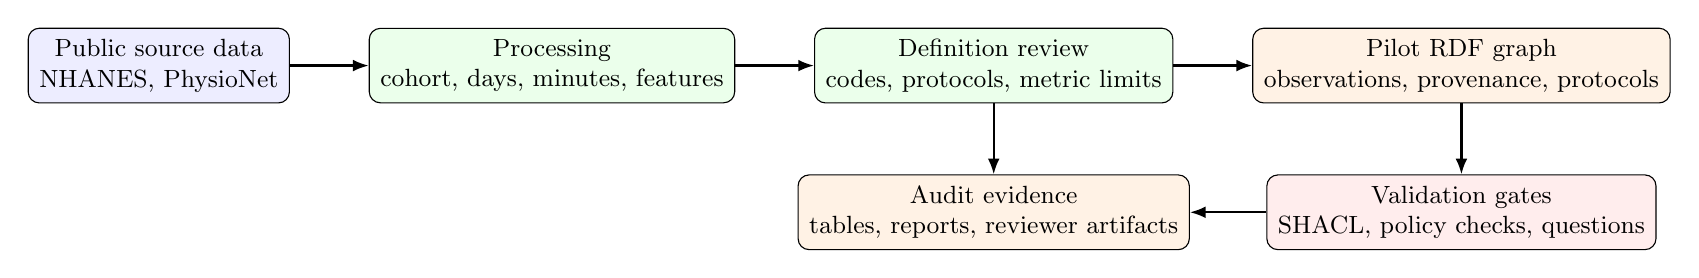
\begin{tikzpicture}[
    node distance=9mm and 10mm,
    box/.style={draw, rounded corners, align=center, inner sep=4pt, font=\small, minimum height=8mm},
    data/.style={box, fill=blue!7},
    proc/.style={box, fill=green!8},
    graph/.style={box, fill=orange!10},
    guard/.style={box, fill=red!7},
    arrow/.style={-{Latex[length=2mm]}, thick}
]
\node[data] (raw) {Public source data\\NHANES, PhysioNet};
\node[proc, right=of raw] (pipeline) {Processing\\cohort, days, minutes, features};
\node[proc, right=of pipeline] (mapping) {Definition review\\codes, protocols, metric limits};
\node[graph, right=of mapping] (kg) {Pilot RDF graph\\observations, provenance, protocols};
\node[guard, below=of kg] (validate) {Validation gates\\SHACL, policy checks, questions};
\node[graph, below=of mapping] (outputs) {Audit evidence\\tables, reports, reviewer artifacts};
\draw[arrow] (raw) -- (pipeline);
\draw[arrow] (pipeline) -- (mapping);
\draw[arrow] (mapping) -- (kg);
\draw[arrow] (kg) -- (validate);
\draw[arrow] (validate) -- (outputs);
\draw[arrow] (mapping) -- (outputs);
\end{tikzpicture}%
}
\caption{Data to graph workflow. Public files are processed into reproducible tables, mapped into reviewed definitions, checked with validation gates, and exported as audit evidence.}
\label{fig:pipeline}
\end{figure*}

The ontology used SOSA style patterns for accelerometer observations and PROV style links for source files, software executions, and generated artifacts. Project terms were added for movement summaries, processing protocols, protocol results, compatibility decisions, and interpretation limits. The pilot graph was limited to 20 selected participants, up to 3 days per participant, up to 5 minute observations per day, and 20 independent PAM daily summaries. This kept the review graph inspectable while the processed tables preserved the full analytic cohort.

\subsection{Harmonisation and terminology review}

Harmonisation was treated as a reviewed claim. Each source variable was assigned one of four compatibility statuses. A source specific metric can be represented but not converted to another metric. A protocol abstraction can be compared only as a completeness rule after its executable condition is represented. A broad construct can group variables under a general concept such as movement volume while blocking numeric equivalence. A not harmonisable status blocks transferred thresholds or activity definitions.

NHANES cancer type values were also treated conservatively. They are self reported source codes, not registry diagnoses. A draft mapping to NCI Thesaurus was reviewed using two expert review files. The completed spreadsheet contained 33 rows. Twenty five rows were approved for qualified graph assertions, while eight were not asserted because they required more information, revision, rejection, or lacked completed approval. The graph stores reviewed NCIt IRIs only as qualified mapping metadata from self reported source codes. It does not assert histology, stage, treatment, recurrence, metastatic status, current disease status, or registry confirmed diagnosis.

\subsection{Validation and competency questions}

Validation had three layers. Required property checks confirmed that graph resources had expected identifiers, source links, protocol links, measurement values, and provenance. pySHACL then checked the RDF graph against the project shapes. Policy guards checked domain rules, including NCIt review status, the number of qualified NCIt assertions, and the absence of unsupported activity classification claims.

Nine competency questions were executed over the generated artifacts. They tested protocol discordance, protocol review status, NCIt mapping qualification, provenance traversal, minute measurement context, self reported cancer history wording, harmonisation compatibility, protocol citation provenance, and independent PAM source validation. These questions were chosen because they match the main reviewer risks: hidden cohort filters, unclear provenance, unsupported cancer terminology claims, and invalid metric conversion.

\section{Results}
\label{sec:results}

\subsection{The same cohort changed under different valid day rules}

The primary NHANES 2011--2014 pipeline retained 1,035 adults with self reported cancer history, including 878 with daily and minute level accelerometry. The retained minute table contained 9,949,908 rows, and the derived participant day feature table contained 7,785 rows. Quality checks passed for participant uniqueness and foreign key consistency.

Valid day definitions changed the analytic cohort (Table~\ref{tab:sensitivity}). Eligible participant counts ranged from 722 under the 12 hour wake wear rule to 862 under the 20 hour valid minutes rule. The largest pairwise discordance was 142 participants, or 16.2 percentage points. This directly supports the motivating claim: the same source cohort can lead to different analytic conclusions because the definition changed.

\begin{table}[t]
\caption{Outcome sensitivity under three valid day completeness rules. MIMS values are movement summary metrics only.}
\label{tab:sensitivity}
\centering
\scriptsize
\begin{tabularx}{\columnwidth}{>{\raggedright\arraybackslash}p{0.42\columnwidth}rrr}
\toprule
Protocol & Eligible & Eligible \% & Valid days \\
\midrule
\shortstack[l]{\texttt{wake\_wear}\\\texttt{10h\_min4}} & 807 & 91.9 & 5,553 \\
\shortstack[l]{\texttt{wake\_wear}\\\texttt{12h\_min4}} & 722 & 82.2 & 4,824 \\
\shortstack[l]{\texttt{valid\_minutes}\\\texttt{20h\_min4}} & 862 & 98.2 & 6,111 \\
\bottomrule
\end{tabularx}
\end{table}

Mean participant daily MIMS also varied by rule: 11,567.6 for the 10 hour wake wear rule, 12,201.5 for the 12 hour rule, and 10,827.1 for the 20 hour valid minutes rule. The graph records these as protocol specific results rather than as one universal activity estimate.

\subsection{The pilot graph passed structural and policy validation}

The rebuilt pilot graph contained 9,324 triples. It represented 20 participants, 25 cancer diagnosis slots, 20 cancer history assertions, 60 daily movement summaries, 300 minute observations, 60 derived feature sets, 3 processing protocols, 60 protocol application results, 12 protocol citation evidence nodes, 4 activity data sources, 9 harmonisation source variable mappings, 4 harmonised activity definitions, 60 synthetic daily activity summaries, and 20 independent PAM daily summaries.

The graph passed pySHACL validation with 5,071 local required property checks, zero failed checks, and zero failed policy checks. The NCIt review guard reported status \texttt{review\_completed\_qualified\_assertions\_allowed} and 19 qualified NCIt assertions in the selected pilot graph (Table~\ref{tab:kgvalidation}).

\begin{table}[t]
\caption{Pilot graph validation summary.}
\label{tab:kgvalidation}
\centering
\small
\begin{tabular}{lr}
\toprule
Measure & Value \\
\midrule
RDF triples & 9,324 \\
Participants & 20 \\
Cancer diagnoses & 25 \\
Daily movement summaries & 60 \\
Minute observations & 300 \\
Processing protocols & 3 \\
Harmonisation mappings & 9 \\
pySHACL conforms & true \\
Validation failed checks & 0 \\
Failed policy checks & 0 \\
Qualified NCIt assertions & 19 \\
\bottomrule
\end{tabular}
\end{table}

\subsection{Unsupported harmonisation claims were made explicit}

The harmonisation layer represented nine source variable mappings across wrist MIMS, synthetic hip counts, independent NHANES PAM counts, and step metrics. Representative decisions are shown in Table~\ref{tab:compatibility}. The graph allowed broad construct level comparison where defensible, but blocked numeric conversion and transferred intensity classification.

\begin{table*}[t]
\caption{Representative harmonisation compatibility decisions.}
\label{tab:compatibility}
\centering
\small
\setlength{\tabcolsep}{4pt}
\begin{tabularx}{\textwidth}{>{\raggedright\arraybackslash}p{0.24\textwidth}>{\raggedright\arraybackslash}p{0.15\textwidth}>{\raggedright\arraybackslash}p{0.10\textwidth}>{\raggedright\arraybackslash}p{0.17\textwidth}Y}
\toprule
Source & Variable & Unit & Compatibility & Interpretation limit \\
\midrule
NHANES 2011--2014 wrist MIMS & PAXMTSD & MIMS & Source specific metric & Do not apply hip counts per minute intensity thresholds to MIMS. \\
NHANES 2011--2014 wrist MIMS & PAXWWMD & minutes & Protocol abstraction & Completeness rule only; not an activity classification. \\
Synthetic hip counts demo & MVPA minutes by 1952 cpm & minutes & Not harmonisable & Requires hip counts per minute protocol context. \\
NHANES 2003--2006 hip PAM & PAXINTEN & counts/min & Broad construct only & Do not convert hip ActiGraph counts to wrist MIMS. \\
NHANES 2005--2006 hip PAM & PAXSTEP & steps/min & Source specific step metric & Steps cannot be inferred from NHANES wrist MIMS. \\
\bottomrule
\end{tabularx}
\end{table*}

A naive pipeline could align these variables by similar labels. The graph instead records that MIMS, steps, and hip counts are different source metrics. It also records that valid wear rules are completeness definitions, not activity status definitions.

\subsection{Comparison sources exposed where harmonisation should stop}

The PhysioNet ActiLife step source had 100\% metadata overlap with the 1,035 NHANES 2011--2014 participants with self reported cancer history. It was modelled as a real same cohort derived source, not as an independent validation cohort. Descriptive paired comparison with MIMS is therefore allowed, but conversion validation is not.

The independent NHANES 2003--2006 hip worn ActiGraph PAM source included 892 adults with self reported cancer history, 768 participants with raw PAM minute records, 5,367 daily summary rows, and 7,724,170 retained minute rows. It provides a stronger cross source test because it differs by cycle, participant set, placement, and metric. The graph includes 20 independent PAM daily summary nodes and competency query evidence that these summaries are source specific and not convertible to wrist MIMS.

\subsection{Activity definitions changed classification within a valid source context}

The NHANES 2003--2006 hip ActiGraph source was used for a definition comparison experiment within the metric for which the rules were defined. Among 768 evaluated participants, 722 met the 10 hour and 12 hour valid day rules. When hip count MVPA definitions were applied within their source context, 457 participants had at least 30 minutes under a 760 counts per minute rule, 58 under a 2020 counts per minute rule, and 11 under a 2020 counts per minute bouted rule. This is not a MIMS conversion. It shows that even within an appropriate source metric, methodological definitions can materially change activity classification.

\subsection{Competency questions produced audit evidence}

The nine competency questions returned expected evidence rows. CQ1 returned 40 rows showing protocol discordant inclusion. CQ5 returned 300 minute observation rows with MIMS, wear state, and quality context. CQ7 returned compatibility evidence. CQ9 returned 20 independent PAM source validation rows. The competency query layer turns reviewer concerns into executable checks rather than narrative assurances.

\section{Discussion}
\label{sec:discussion}

\subsection{Principal interpretation}

This study starts from a practical problem: the same survivor can lead to different activity related conclusions because the method changed. The results show that this is not hypothetical. In the NHANES cancer history cohort, valid day rules changed eligible participant counts by 16.2 percentage points. In the independent hip ActiGraph source, activity definitions produced very different counts of participants meeting a 30 minute MVPA criterion. These differences are methodological facts that should be visible to reviewers and downstream users.

The knowledge graph contribution is to make those methodological facts inspectable. A processed table can report the number 722 or 862, but it does not itself explain the protocol, source metric, review status, or blocked interpretations behind the number. The graph represents these definitions as linked evidence. It also makes negative knowledge explicit. The system can say not only what a variable is, but also what it must not be used to claim.

\subsection{Why the cancer domain matters}

Cancer survivorship is a high value and high risk domain for this kind of semantic audit. It is high value because physical activity is relevant to survivorship care, functional recovery, fatigue, and long term health outcomes \cite{rock2022acs,schmitz2019exercise}. It is high risk because survivors are heterogeneous and because public survey cancer variables often lack clinical depth. A method that silently changes who is eligible or how activity is classified can change the interpretation of group comparisons and may affect how evidence is reused.

The graph therefore applies caution in two places. First, accelerometer variables are kept tied to their device placement, metric, and protocol. Second, cancer type mappings are kept tied to self reported NHANES source codes. Expert review can support terminology alignment, but it does not turn a survey response into histology, stage, recurrence, treatment, metastatic status, or current disease status.

\subsection{Implications for knowledge engineering automation}

For knowledge engineering automation, the main lesson is that automation should not hide expert judgement. It should capture it. The pipeline converts repeated decisions into artifacts: source manifests, protocol definitions, mapping tables, NCIt review decisions, SHACL shapes, policy guards, competency questions, and risk reports. This supports reproducibility because the same definitions can be rerun. It supports accountability because the limits of each definition are stated in the graph.

This is relevant for AI systems that retrieve or reason over knowledge graphs. If a graph contains only positive links, an AI workflow may generate plausible but invalid harmonisation claims. If the graph also contains compatibility statuses and interpretation limits, retrieval augmented and agent based workflows can be constrained by explicit domain rules rather than by prompt wording alone.

\subsection{Comparison with label based harmonisation}

A label based harmonisation workflow might group MIMS, steps, hip counts, MVPA minutes, and valid wear under physical activity. That may be useful for search, but it is not sufficient for analysis. The current framework separates broad conceptual grouping from analytic equivalence. This lets users discover related variables while preventing invalid conversion or threshold transfer.

The same principle applies to cancer terminology. Mapping a source label to NCIt can improve search and interoperability, but the mapping must preserve the strength of the source evidence. In this study, reviewed NCIt IRIs are qualified mappings from self reported code labels, not diagnosis assertions about participants.

\subsection{Limitations}

The current implementation is a pilot. The RDF graph is limited to selected participants, days, and minute observations, although the processed tables cover all retained participants. NHANES cancer history is self reported, so the cohort should not be described as registry confirmed survivorship. NCIt mapping review is complete with caveats, but reviewed IRIs remain qualified mappings from source codes. The external domain and ontology review of accelerometer source independence, metric compatibility, valid day interpretation, and graph modelling claims is prepared but still pending completion. A public reproducibility archive with DOI has not yet been deposited. Finally, the graph validates structure and policy gates; it does not evaluate large scale reasoning performance.

\subsection{Future work}

Future work should scale the graph beyond the pilot selection, deposit the reproducibility archive with a persistent DOI, complete external domain and ontology review, and add datasets with clinically verified diagnosis, treatment, stage, recurrence, and outcome variables. Methodologically, the framework can be extended to extract protocol definitions from papers with AI support, provided that extracted rules pass the same review and validation gates.

\section{Conclusion}
\label{sec:conclusion}

Different accelerometer definitions can change who enters a cancer survivorship analysis and how activity is interpreted. This paper showed how those definitions can be represented as auditable knowledge graph objects rather than hidden preprocessing choices. In NHANES adults with self reported cancer history, valid day rules changed eligible participant counts from 722 to 862. The pilot graph passed SHACL and policy validation, preserved provenance, represented expert reviewed cancer terminology mappings conservatively, and blocked unsupported harmonisation across wrist MIMS, steps, and hip counts. The practical conclusion is that cancer survivorship accelerometry studies should make methodological definitions explicit, queryable, and reviewable before their results are reused in clinical, epidemiological, or AI workflows.

\section*{Data and code availability}

The source datasets used in this study are public NHANES and PhysioNet resources. NHANES files are available from the US National Center for Health Statistics NHANES public data portal. PhysioNet minute level step count and physical activity data from NHANES 2011--2014 are available as version 1.0.2 with DOI 10.13026/d7sw-f662. The current project contains generated processed artifacts, validation reports, and manuscript tables. Consistent with FAIR data stewardship principles \cite{wilkinson2016fair}, a repository or archive DOI for the full reproducibility bundle should be added before submission: \todo{insert Zenodo/OSF/GitHub DOI or permanent URL}. Public source URLs and access dates should be supplied in the online submission data statement rather than added to the bibliography, because this manuscript restricts bibliographic references to Scopus indexed scholarly publications.

\section*{Ethics statement}

This study uses public, deidentified NHANES and PhysioNet data and does not collect new human subject data. The cohort is described as adults with self reported cancer history; no registry confirmed diagnosis, treatment, recurrence, metastatic status, or current disease status is inferred.

\section*{Funding}

This research did not receive any specific grant from funding agencies in the public, commercial, or not for profit sectors. \todo{Confirm before submission.}

\section*{Declaration of competing interest}

The authors declare that they have no known competing financial interests or personal relationships that could have appeared to influence the work reported in this paper. \todo{Confirm for all authors before submission.}

\section*{CRediT authorship contribution statement}

\todo{Complete after final author list is fixed. Suggested roles: Conceptualization, Methodology, Software, Data curation, Formal analysis, Validation, Visualization, Writing -- original draft, Writing -- review and editing, Supervision.}

\section*{Declaration of generative AI and AI assisted technologies in the manuscript preparation process}

During the preparation of this work the author(s) used OpenAI ChatGPT/Codex to support manuscript drafting, LaTeX organization, and consistency checking against generated project artifacts. After using this tool, the author(s) reviewed and edited the content as needed and take full responsibility for the content of the submitted article.

\section*{Acknowledgements}

We thank Christos Kazazis, MD, specialist doctor in Internal Medicine and Diabetology, Department of History of Medicine and Medical Ethics, National and Kapodistrian University of Athens, Athens, Greece, for expert review of the NHANES cancer code to NCI Thesaurus mapping spreadsheet.

We thank Helena Linardou, MD PhD, Medical Oncologist and Director of the 4th Oncology Department and Clinical Trials Center, Metropolitan Hospital, Athens, Greece, for clinical review of the cancer code mapping strategy and interpretation limits.

These acknowledgements recognize expert review input only. The mapped NHANES cancer type codes remain self reported source code mappings and should not be interpreted as registry confirmed diagnoses, histology confirmations, staging, treatment, recurrence, or current disease status assertions.

\appendix

\section{Competency questions}
\label{app:cq}

\begin{table*}[t]
\caption{Competency questions used for reviewer validation.}
\label{tab:cq}
\centering
\small
\begin{tabularx}{\textwidth}{>{\raggedright\arraybackslash}p{0.08\textwidth}>{\raggedright\arraybackslash}p{0.24\textwidth}rY}
\toprule
ID & Purpose & Rows & Reviewer risk addressed \\
\midrule
CQ1 & Protocol discordance & 40 & Protocol choice changes inclusion. \\
CQ2 & Protocol review status & 3 & Protocols are reviewed completeness rules. \\
CQ3 & Reviewed cancer mappings & 25 & NCIt mappings are qualified and not overinterpreted. \\
CQ4 & Daily feature provenance & 60 & Movement features expose provenance. \\
CQ5 & Minute measurement context & 300 & MIMS, wear state, and quality context are queryable. \\
CQ6 & Self reported cancer history & 20 & Cohort is not overclaimed as clinically verified survivorship. \\
CQ7 & Harmonisation compatibility & 13 & Compatibility and incompatibility are queryable. \\
CQ8 & Protocol citation provenance & 12 & Protocol evidence and support levels are queryable. \\
CQ9 & Independent PAM source validation & 20 & Independent PAM evidence and non conversion limits are queryable. \\
\bottomrule
\end{tabularx}
\end{table*}

\section{Current submission readiness gates}
\label{app:gates}

Before final submission, the remaining gates are: (i) completion of the external domain and ontology review sheet for accelerometer source independence, metric compatibility, valid day interpretation, and graph modelling pattern; (ii) deposit of a reproducibility archive with DOI; and (iii) completion of the final target journal reporting checklist and author metadata.

\bibliographystyle{elsarticle-num}
\bibliography{references}

\end{document}
